In this section we will present the results of the benchmarks executed on the anonymization algorithm, and compare the results to the expected algorithm characteristics introduced earlier in Chapter~\ref{ch:chapter_algorithm}. As mentioned in Section~\ref{subsec:benchmarks} benchmarks in Go are special tests, which can be executed with the testing framework. Go will help us run the analyzed function until the measure is \emph{stable}, and is able to precisely calculate the average execution time.

\subsection{Test Rig}

The configuration that was used for executing the benchmarks is summarized on Figure~\ref{fig:test_rig}.
\begin{figure}[H]
    \centering
    \small
    \begin{tabular}{r l}
        \toprule
        Operating System Kernel        & Linux 5.3.1-arch \\
        CPU Model                      & Intel® Pentium® G4620 @ 3.70GHz \\
        CPU Cores                      & 2 \\
        Total Memory                   & 16335268 kB \\
        Go Version                     & go1.13 linux/amd64 \\
        Anonymizer Version             & 1.2.7 \\
        \bottomrule
    \end{tabular}
    \caption{Benchmark test rig}\label{fig:test_rig}
\end{figure}

\subsection{RangeGeneralizer benchmarks}\label{subsec:range_generalizer_benchmarks}

Figure~\ref{fig:range_bm} shows a comparison benchmark of both range based generalizers --- \texttt{IntRange} and \texttt{FloatRange}. The horizontal axis plots the size of the range, the vertical axis shows the \emph{average time to generalize the median value in the range to the highest level} in nanoseconds as measured by the Go bench framework. As expected, both show a \textbf{logarithmic} progression curve (note the logarithmic scale on the horizontal axis). Generalizing float ranges is more expensive however, this is due to the increased number of splits and additional cost of comparison with delta.

\vspace{\baselineskip}
\begin{figure}[ht]
    \centering
    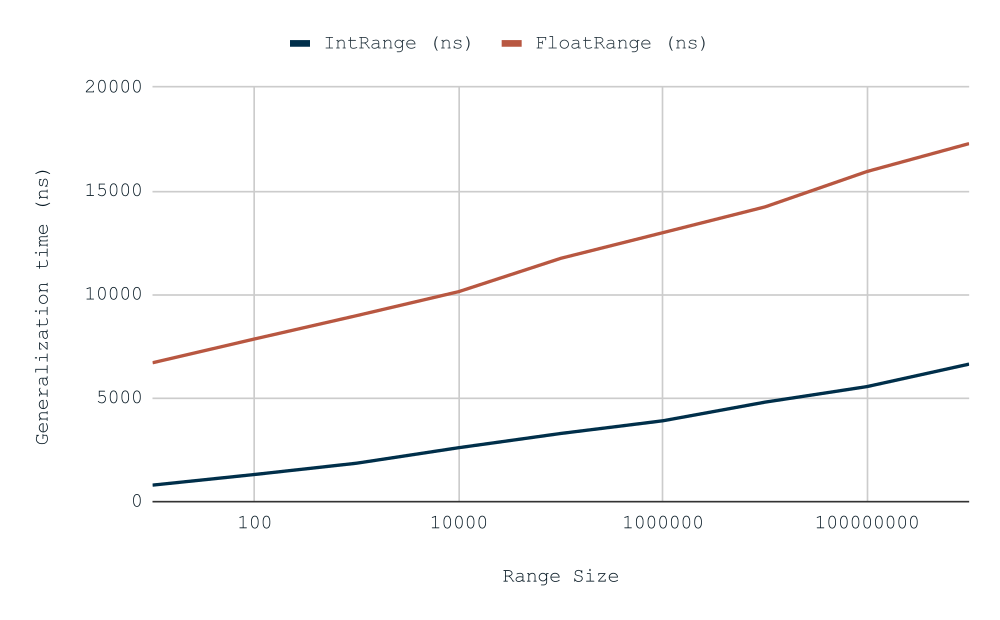
\includegraphics[width=0.8\textwidth]{images/range.png}
    \caption{Range Generalizer Benchmarks}\label{fig:range_bm}
\end{figure}

\subsection{PrefixGeneralizer benchmarks}

The \texttt{PrefixGeneralizer} has three different parameters. For each benchmark, we will test one parameter while the other two are fixed. The tests always generalize the input to the \emph{maximum possible level}.

\subsubsection{Word Count}

In this test we set the maximum allowed words to a high enough fixed value, and benchmark the performance based on the \emph{actual number of words} (amount of text) on the input of the generalizer. Figure~\ref{fig:prefix_word_count_bm} shows a relatively flat \textbf{exponential curve}. The performance starts to degrade after 5000 words, which is an indicator of the amount of (English) text it is supposed to be able to handle per cell in the input data table.

\vspace{\baselineskip}
\begin{figure}[H]
    \centering
    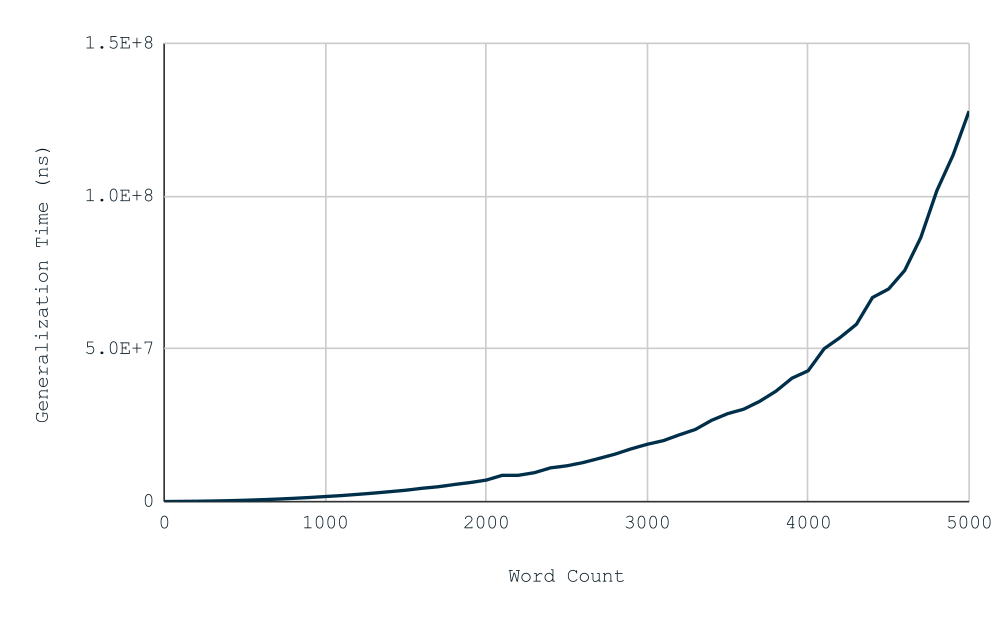
\includegraphics[width=0.8\textwidth]{images/prefix-word-count.png}
    \caption{Prefix --- Word Count Benchmark}\label{fig:prefix_word_count_bm}
\end{figure}

\subsubsection{Word Length}

As discussed during the introduction of the prefix generalizer in Section~\ref{subsec:prefix_generalizer} the performance of the prefix generalization algorithm should be \emph{unaffected} by the length of words. The benchmark on Figure~\ref{fig:prefix_word_length_bm} proves this adequately. The time needed to generalize with fixed max words, word count and increasing word length assumes a \textbf{flat line}.

\vspace{\baselineskip}
\begin{figure}[H]
    \centering
    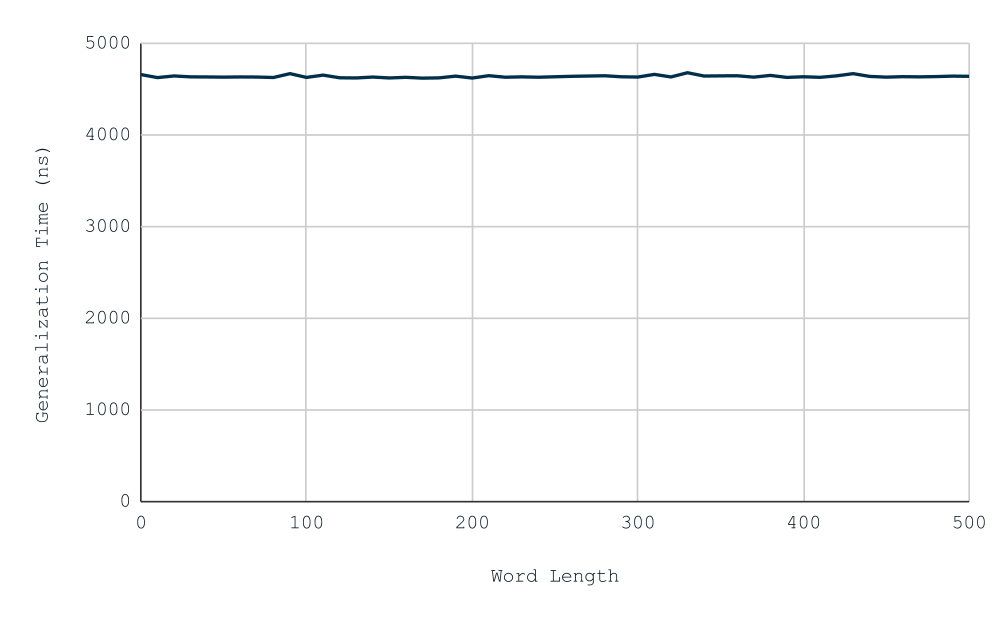
\includegraphics[width=0.8\textwidth]{prefix-word-length.png}
    \caption{Prefix --- Word Length Benchmark}\label{fig:prefix_word_length_bm}
\end{figure}

\subsubsection{Max Words}

Finally we inspect the effect of the \texttt{MaxWords} parameter. We can recall, that this parameter increases the \emph{total levels} of the generalizer, even when the actual number of words in the generalized text is smaller. Thus the \textbf{linear curve} visible on Figure~\ref{fig:prefix_max_words_bm} seems realistic.

\vspace{\baselineskip}
\begin{figure}[H]
    \centering
    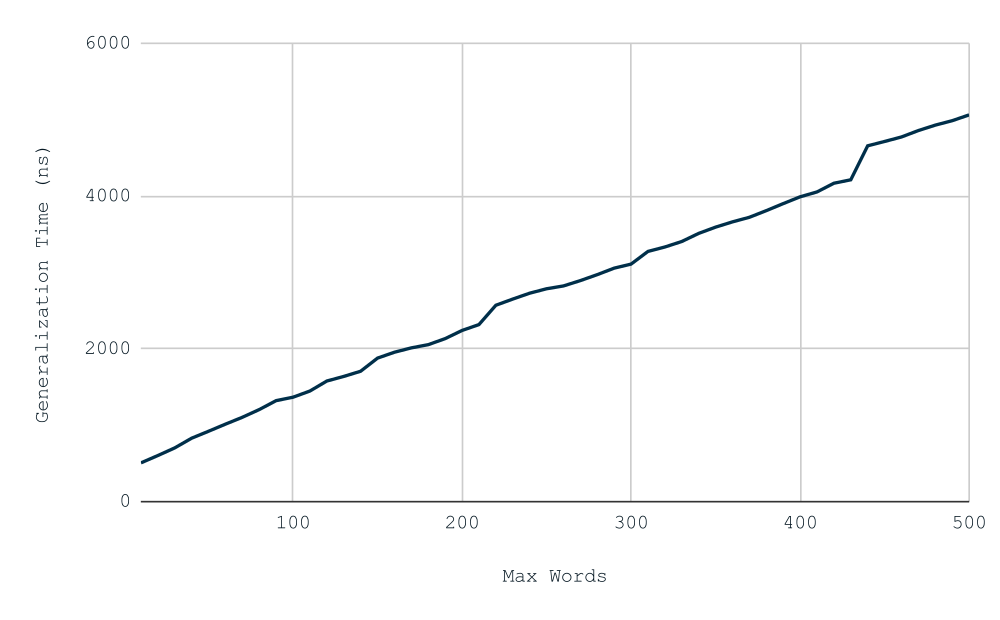
\includegraphics[width=0.8\textwidth]{images/prefix-max-words.png}
    \caption{Prefix --- Max Words Benchmark}\label{fig:prefix_max_words_bm}
\end{figure}

\subsection{HierarchyGeneralizer benchmarks}

\subsubsection{Hierarchy depth}
One way hierarchies can be benchmarked is based on their depth. Given a fixed node count, the number of levels correlates to the number of children each node in the hierarchy has. Since it is easier to build a hierarchy by specifying the number of children per node, we will use this approach for our benchmark. Figure~\ref{fig:hierarchy_children_bm} shows an interesting result (note the logarithmic vertical axis). The generalization time greatly improves with a more flat hierarchy up to around 4 or 5 children. Increasing the child-count further has no significant beneficial effect. The explanation for this behavior is, that while the generalization hierarchy is not actually a search-tree, increasing the child-count thus reducing the total number of levels for the same amount of nodes will actually improve the number of steps needed to locate the partition a given item belongs to on a certain level (up to a certain threshold).
\vspace{\baselineskip}
\begin{figure}[H]
    \centering
    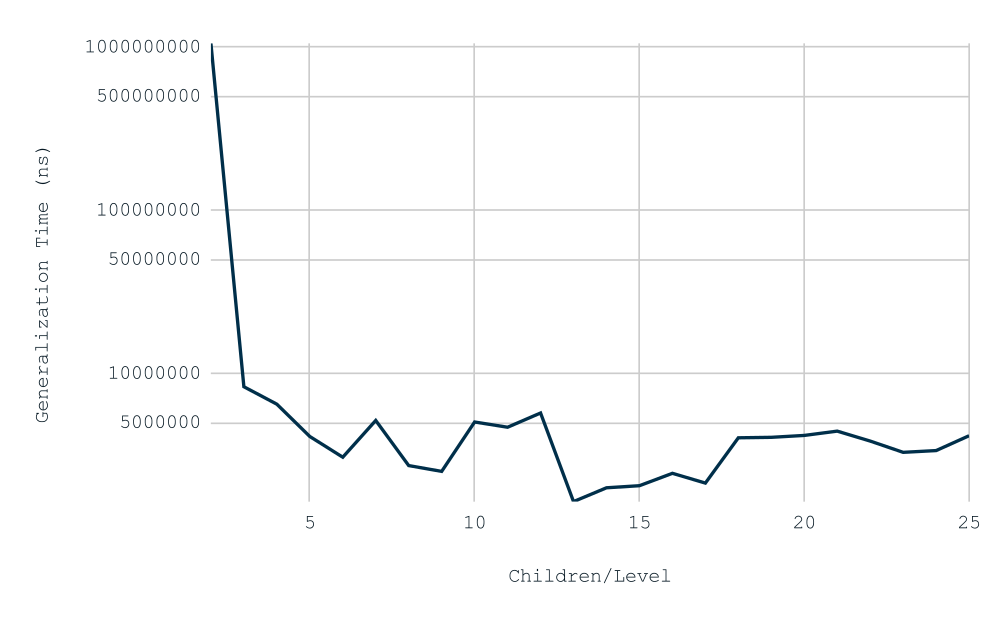
\includegraphics[width=0.8\textwidth]{hierarchy-children.png}
    \caption{Hierarchy --- Children per Node Benchmark}\label{fig:hierarchy_children_bm}
\end{figure}

\subsubsection{Number of nodes}
By increasing the number of nodes in the hierarchy, the generalization time will increase in a \textbf{linear} fashion as shown on Figure~\ref{fig:hierarchy_nodes_bm}.
\vspace{\baselineskip}
\begin{figure}[H]
    \centering
    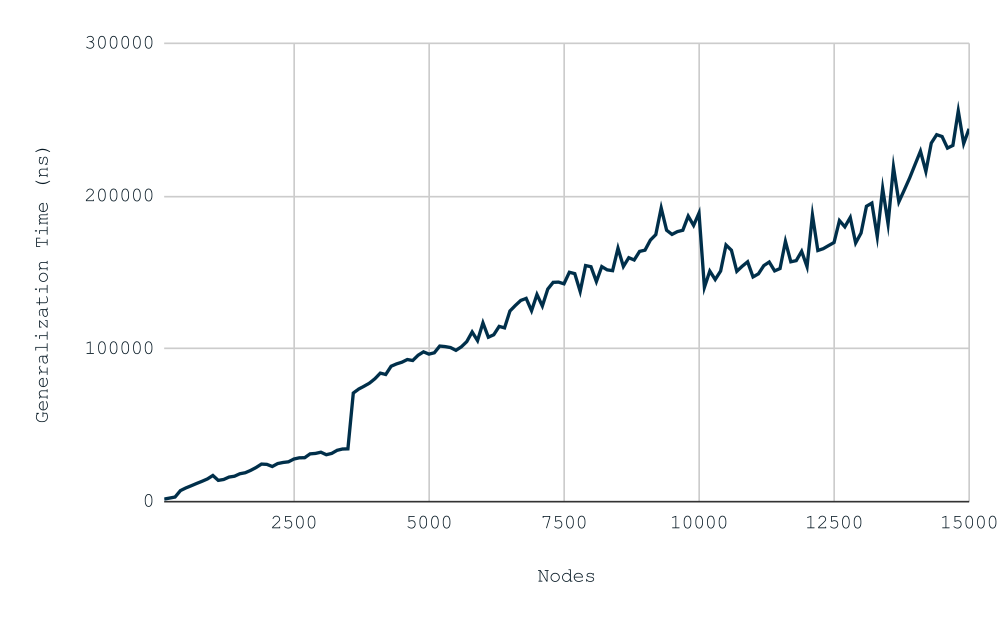
\includegraphics[width=0.8\textwidth]{images/hierarchy-nodes.png}
    \caption{Hierarchy --- Number of Nodes Benchmark}\label{fig:hierarchy_nodes_bm}
\end{figure}

\subsection{Comparison of generalizers}

Plotting all the built-in generalizers on the same chart gives a good opportunity to compare their relative performance when the row count is being increased given a fixed set of parameters. Note, that each generalizer has several different parameters which affect the performance greatly, so the following comparisons are only approximate guidelines.

According to Figure~\ref{fig:compare_all} the slowest generalizer is the \texttt{FloatRange} generalizer. This might be a surprise in light of Section~\ref{subsec:range_generalizer_benchmarks}, which showed that the numeric range generalizers scaled really well, when considering only the parameter which controls the width of the range. Unfortunately, when having a large amount of numeric columns with a fixed range width, they have a poor performance when the number of rows in the table is increased. 

In order to get a better overview, Figure~\ref{fig:compare_fast} shows the same setup with \texttt{FloatRange} omitted.

\vspace{\baselineskip}
\begin{figure}[ht]
    \centering
    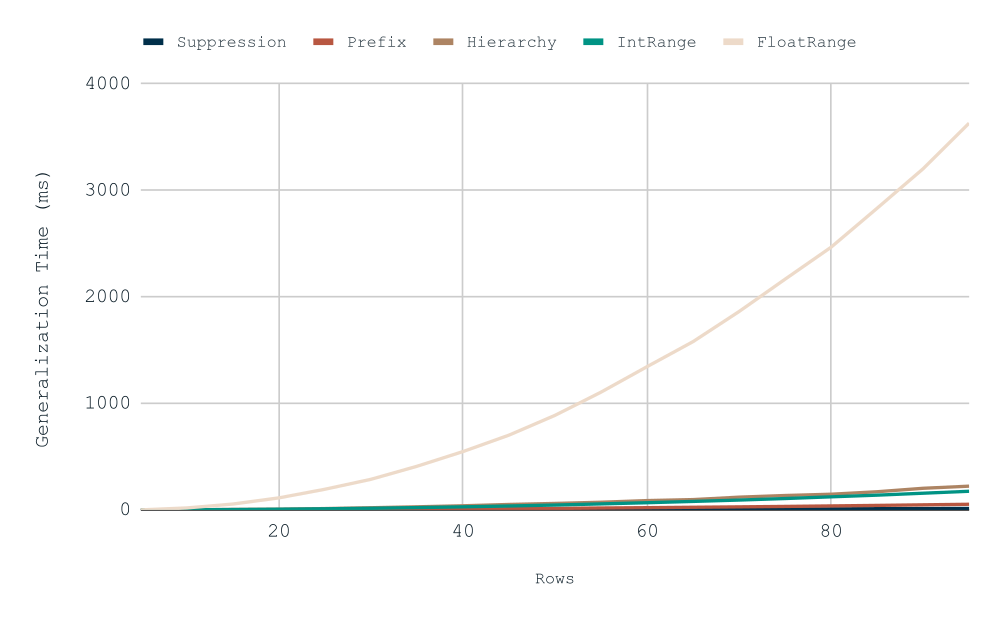
\includegraphics[width=0.8\textwidth]{images/compare-all.png}
    \caption{Generalizer Speed Comparison}\label{fig:compare_all}
\end{figure}

\vspace{\baselineskip}
\begin{figure}[H]
    \centering
    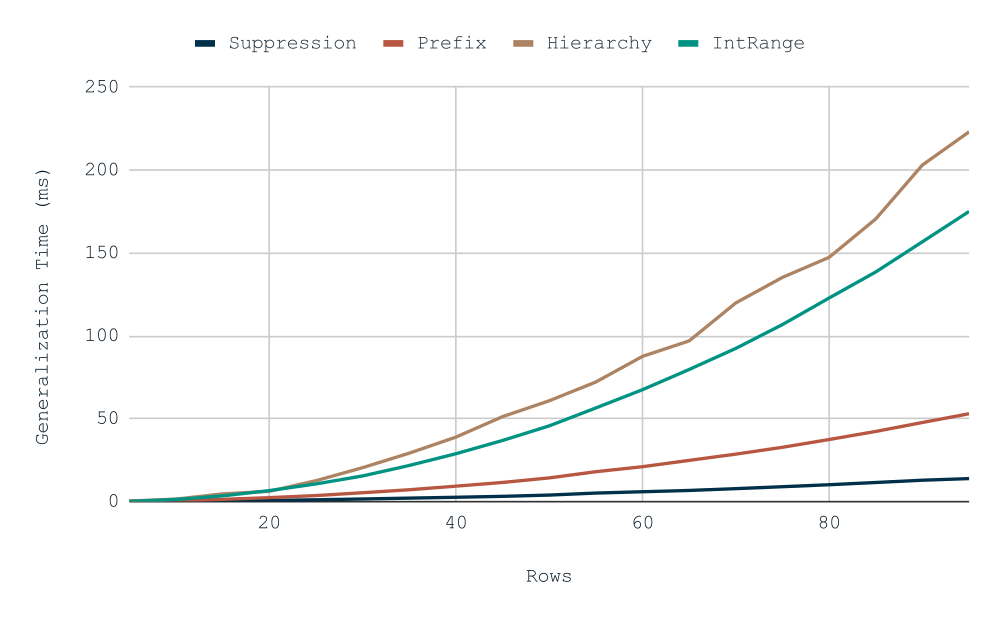
\includegraphics[width=0.8\textwidth]{images/compare-fast.png}
    \caption{Generalizer Speed Comparison (without FloatRange)}\label{fig:compare_fast}
\end{figure}

\subsection{Anonymization benchmarks}

The following benchmarks measure the anonymization of a full sample data table. The table contains only integer numbers generalized with the same \texttt{IntRange} generalizer. The benchmark variables are the \emph{column count}, the \emph{row count} and the \emph{k} anonymity parameter.

\subsubsection{Column count}

We can expect the generalization time to increase for increasing the number of columns in the table. The reason is, that we need to compare more data when calculating the \emph{scaled generalization cost} for the cost-graph. This extra amount of work however is only \textbf{linear}, as shown on Figure~\ref{fig:anon_columns}.

\vspace{\baselineskip}
\begin{figure}[H]
    \centering
    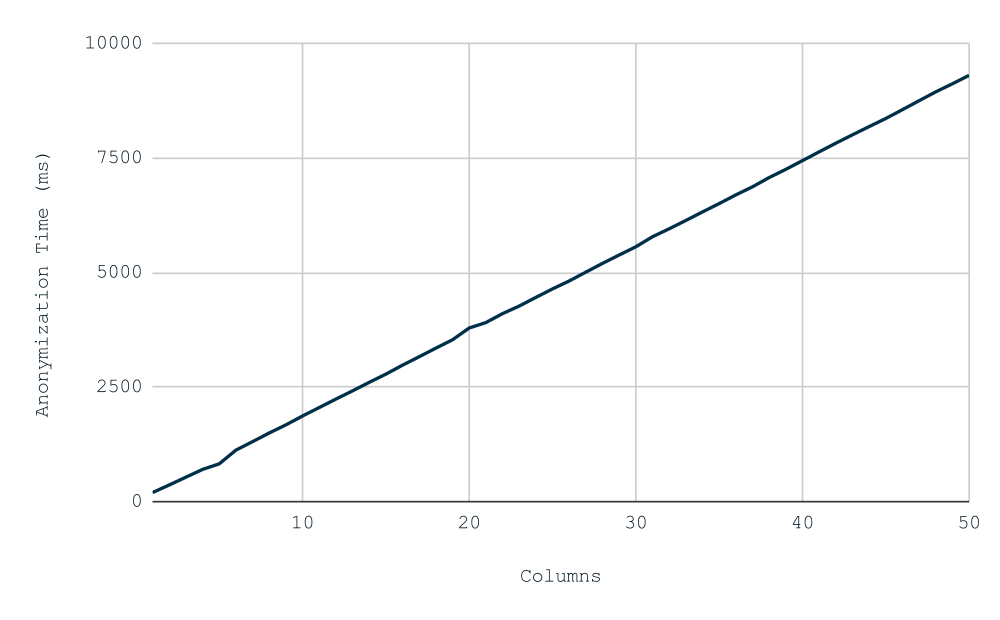
\includegraphics[width=0.8\textwidth]{anon-columns.png}
    \caption{Anonymization vs Column count}\label{fig:anon_columns}
\end{figure}

\subsubsection{Row count}

This is the most important benchmark of all of the above, as it (indirectly) measures the core implementation of the graph based approximation algorithm. As proven in Section~\ref{subsec:polynomial-time-approximation-algorithm} increasing the number of rows in the table should result in a \(\mathcal{O}(kn^2)\) curve. The benchmark on Figure~\ref{fig:anon_rows} confirms, that \textbf{our implementation of the algorithm has the same characteristics}.

\vspace{\baselineskip}
\begin{figure}[ht]
    \centering
    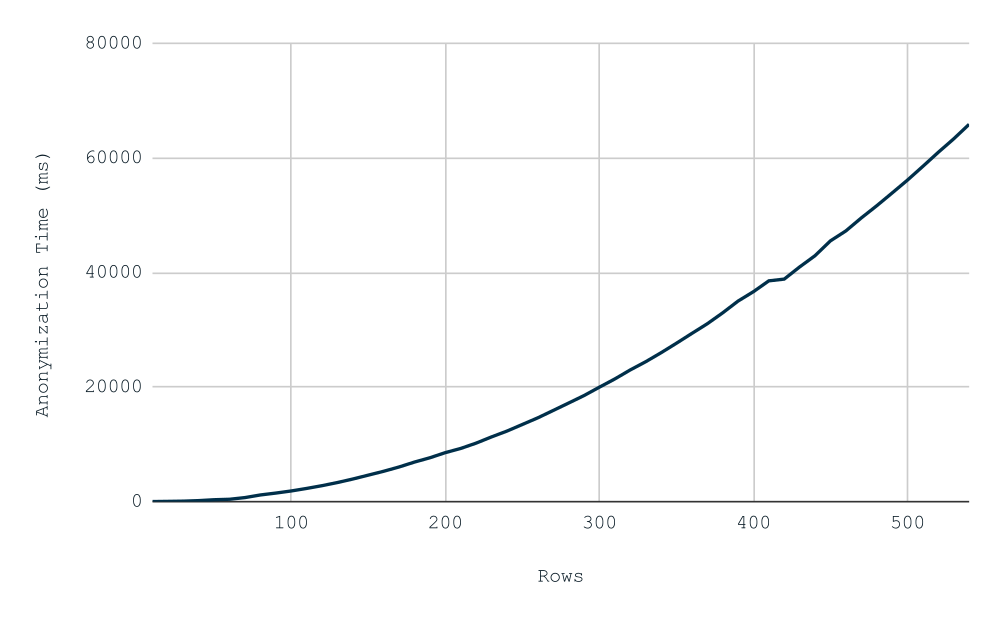
\includegraphics[width=0.8\textwidth]{anon-rows.png}
    \caption{Anonymization vs Row count}\label{fig:anon_rows}
\end{figure}

\subsubsection{k value}

Finally, we investigate if the \emph{k} anonymity parameter has any effect on the anonymization time. In this benchmark the \emph{k} value was increased from 2 to 100 while having all other input parameters fixed. The only restriction is, that the data table needs to contain at least \emph{k} number of rows in order to be able to achieve k-anonymity. The resulting benchmark can be seen on Figure~\ref{fig:anon_k} and shows, that the \emph{k} value has no measurable effect on the anonymization time for a static sized input table.

\vspace{\baselineskip}
\begin{figure}[ht]
    \centering
    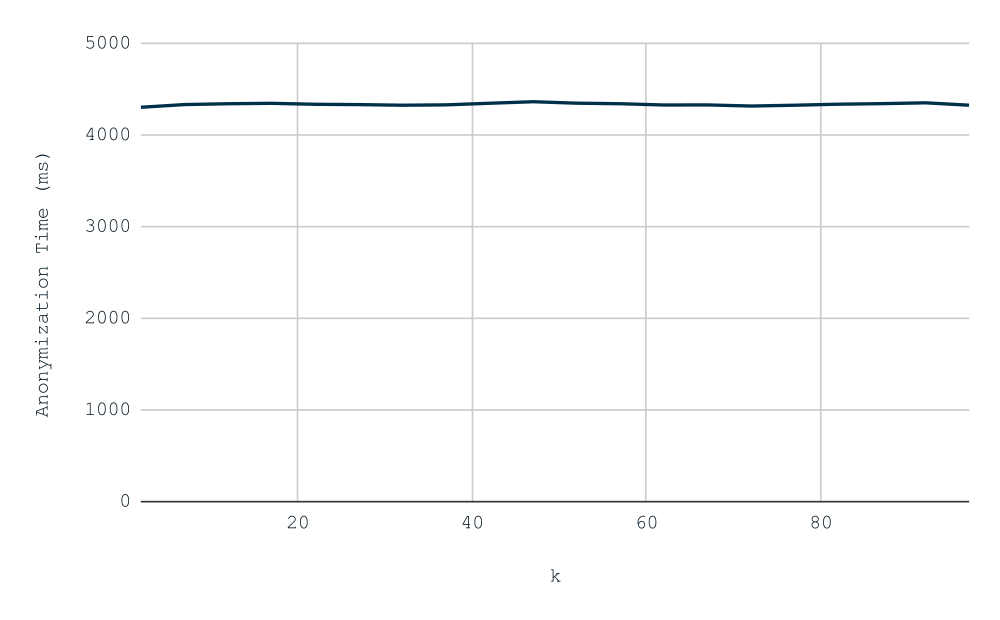
\includegraphics[width=0.8\textwidth]{images/anon-k.png}
    \caption{Anonymization  time vs the \emph{k} anonymity parameter}\label{fig:anon_k}
\end{figure}